\begin{figure}[htb]
  \centering
%segundo bloco de figuras
  \begin{tabular}{c c c c c }
    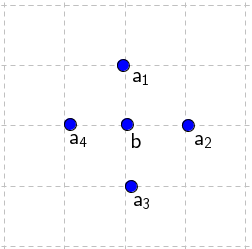
\includegraphics[width=3.5cm]{./img/disposicaoTortaGrid.png}    
    & &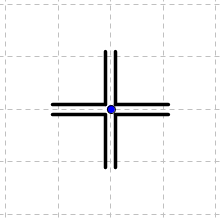
\includegraphics[width=3.5cm]{./img/truePieGrid.png} 
    & &
 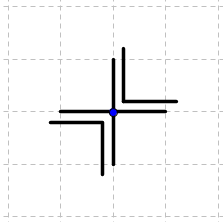
\includegraphics[width=3.5cm]{./img/falsePieGrid.png} \\%[\abovecaptionskip]
    {\footnotesize (a) 4-estrela na grade}  & &  {\footnotesize (b) True pie} & & {\footnotesize (c) False pie} %\label{fig:frame}
  \end{tabular}
  \caption{Representações $B_{1}$-EPG do ciclo induzido de tamanho  4 como tortas, com ponto central $b$}\label{fig:piesInGrid}
\end{figure} 